\documentclass[tikz,border=2pt,11pt]{standalone}
\usetikzlibrary{calc}
\usetikzlibrary{arrows.meta}
\usetikzlibrary{patterns}
\usetikzlibrary{positioning}
\usepackage{amsmath}
\usepackage{amssymb}
\usepackage{mathrsfs}
\usepackage{graphicx}
\usepackage{tikz}
\newcommand{\R}{\mathbb R}
\newcommand{\C}{\mathbb C}
\newcommand{\Z}{\mathbb Z}
\newcommand{\N}{\mathbb N}
\newcommand{\E}{\mathbb E}
\newcommand{\PP}{\mathbb P}
\newcommand{\1}{\mathbf1}
\newcommand{\dd}{\,\mathrm d}
\newcommand{\abs}[1]{\lvert#1\rvert}
\newcommand{\norm}[1]{\lVert#1\rVert}
\newcommand{\ip}[2]{\langle#1,#2\rangle}
\DeclareMathOperator{\Tr}{Tr}
\DeclareMathOperator{\diag}{diag}
\DeclareMathOperator{\dist}{dist}
\DeclareMathOperator{\supp}{supp}
\DeclareMathOperator{\diam}{diam}
\DeclareMathOperator{\rad}{rad}
\DeclareMathOperator{\Div}{div}
\DeclareMathOperator{\Rea}{Re}
\DeclareMathOperator{\Ima}{Im}
\DeclareMathOperator{\Var}{Var}
\DeclareMathOperator{\sech}{sech}
\newcommand{\articleid}[1]{\begingroup\small\ttfamily\hyphenchar\font=45 #1\endgroup}
\begin{document}
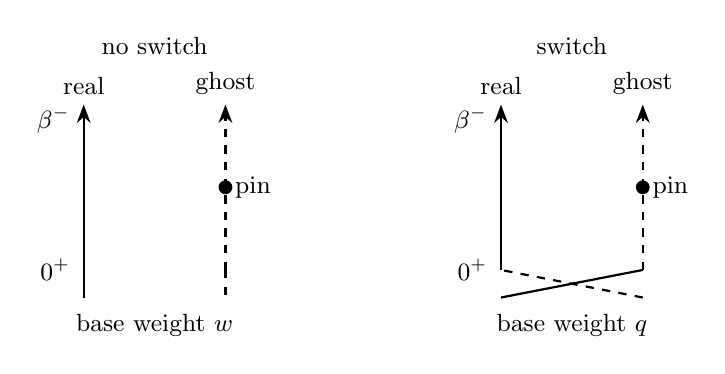
\begin{tikzpicture}[x=1cm,y=1cm,>=Stealth,font=\small]
 \foreach \x/\lab in {0/{no switch},5.3/{switch}} {
  \node at (\x+1.3,3.25) {\lab};
  \draw[->,thick] (\x+.4,.4)--(\x+.4,2.5);
  \draw[->,thick,dashed] (\x+2.2,.4)--(\x+2.2,2.5);
  \node[above] at (\x+.4,2.5) {real};
  \node[above] at (\x+2.2,2.5) {ghost};
  \fill (\x+2.2,1.45) circle (2.5pt);
  \node[right] at (\x+2.2,1.45) {pin};
  \node[left] at (\x+.35,.4) {\(0^+\)};
  \node[left] at (\x+.35,2.3) {\(\beta^-\)};
 }
 \draw[thick] (.4,.4)--(.4,.05);
 \draw[thick,dashed] (2.2,.4)--(2.2,.05);
 \node at (1.3,-.3) {base weight \(w\)};
 \draw[thick] (5.7,.05)--(7.5,.4);
 \draw[thick,dashed] (7.5,.05)--(5.7,.4);
 \node at (6.6,-.3) {base weight \(q\)};
\end{tikzpicture}
\end{document}
